% !TEX root = task-3-18-2.tex
% Editable task bank. Append new BankTask blocks at the end of the document.
\documentclass[12pt,a4paper]{article}
\usepackage{physics-textbook}
\usepackage{graphicx,needspace}
\usetikzlibrary{decorations.pathmorphing}
\newif\ifShowSolutions
\ifdefined\TutorEdition
  \ShowSolutionstrue
\else
  \ShowSolutionsfalse % Change to \ShowSolutionstrue to display solutions.
\fi
\newcounter{banktask}
\newsavebox{\BankTaskBox}
\newcommand{\BankTaskContent}[3]{%
  \noindent\textbf{\thebanktask.}\quad #2\par
  \ifShowSolutions
    \Needspace{50mm}% Keep the solution heading with its opening text or diagram.
    #3\par
    \ifdefined\TutorEdition
      \ifcsname TutorSource#1\endcsname
        \nopagebreak\smallskip{\small\csname TutorSource#1\endcsname\par}%
      \fi
    \fi
  \fi
}
\newcommand{\BankTask}[3]{%
  \refstepcounter{banktask}\par\medskip
  \sbox{\BankTaskBox}{\begin{minipage}{\linewidth}%
    \BankTaskContent{#1}{#2}{#3}\end{minipage}}%
  \ifdim\dimexpr\ht\BankTaskBox+\dp\BankTaskBox\relax>\dimexpr\textheight-20mm\relax
    \Needspace{35mm}\BankTaskContent{#1}{#2}{#3}%
  \else
    \Needspace{\dimexpr\ht\BankTaskBox+\dp\BankTaskBox\relax}%
    \noindent\usebox{\BankTaskBox}\par
  \fi
  \medskip
}
\begin{document}
\BookSubsection{3.18.2}{Сила Ампера}


% Source sdamgia-25779: https://phys-ege.sdamgia.ru/problem?id=25779
\BankTask{sdamgia-25779}{
\begin{center}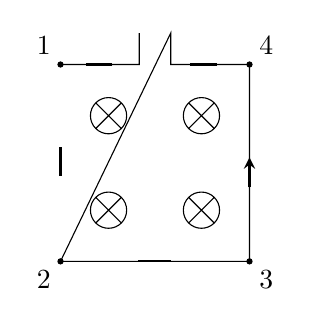
\begin{tikzpicture}[>=stealth]
\draw (0,2.5)--(1,2.5)--(1,2.9) (1.4,2.9)--(1.4,2.5)--(2.4,2.5)--(2.4,0)--(0,0)--cycle;
\draw[->,thick] (.66,2.5)--(.32,2.5) (1.99,2.5)--(1.65,2.5)
 (0,1.45)--(0,1.08) (.99,0)--(1.4,0) (2.4,.94)--(2.4,1.32);
\foreach \x in {.61,1.79}\foreach \y in {.65,1.85}{\draw(\x,\y)circle(.23) (\x-.155,\y-.155)--(\x+.155,\y+.155) (\x-.155,\y+.155)--(\x+.155,\y-.155);}
\fill (0,2.5)circle(.04) (0,0)circle(.04) (2.4,0)circle(.04) (2.4,2.5)circle(.04);
\node[above left] at(0,2.5){$1$};\node[below left] at(0,0){$2$};
\node[below right] at(2.4,0){$3$};\node[above right] at(2.4,2.5){$4$};
\end{tikzpicture}\end{center}
Квадратная рамка с током, направление которого указано на рисунке, помещена в однородное магнитное поле, магнитные линии которого направлены перпендикулярно плоскости рамки от наблюдателя. Как направлена относительно рисунка (вправо, влево, вверх, вниз, к наблюдателю, от наблюдателя) вызванная этим полем сила Ампера, действующая на проводник $2$–$3$? Ответ запишите словом (словами).
}{
\smallskip\noindent\textbf{Решение}\par
По правилу левой руки (магнитные линии входят в ладонь, четыре пальца показывают направление тока в проводнике, большой палец указывает направление силы Ампера) сила Ампера направлена вверх.

Ответ: вверх.
}

% Source sdamgia-1529: https://phys-ege.sdamgia.ru/problem?id=1529
\BankTask{sdamgia-1529}{
Прямолинейный проводник длиной $0{,}5\,\text{м}$, по которому течет ток $6\,\text{А}$, находится в однородном магнитном поле. Модуль вектора магнитной индукции $0{,}2\,\text{Тл}$, проводник расположен под углом $30 ^\circ$ к вектору В. Какова сила, действующая на проводник со стороны магнитного поля?
}{
\smallskip\noindent\textbf{Решение}\par
Сила Ампера, действующая со стороны магнитного поля на проводник с током, определяется выражением:

\[F=IBL \sin \alpha =6\,\text{А} \cdot 0{,}2\,\text{Тл} \cdot 0{,}5\,\text{м} \cdot \sin 30 ^\circ=0{,}3\,\text{Н}.\]

Ответ: $0{,}3$.
}

% Source sdamgia-1534: https://phys-ege.sdamgia.ru/problem?id=1534
\BankTask{sdamgia-1534}{
При силе тока в проводнике $20\,\text{А}$ на участок прямого проводника длиной $50\,\text{см}$ в однородном магнитном поле действует сила Ампера $12\,\text{Н}$. Вектор индукции магнитного поля направлен под углом $37^\circ$ к проводнику $( \sin 37 ^\circ\approx 0{,}6,$ $\cos 37 ^\circ\approx 0{,}8 ) .$ Определите модуль индукции магнитного поля. Выразите модуль индукции в теслах и округлите до целого числа.
}{
\smallskip\noindent\textbf{Решение}\par
Сила Ампера, действующая со стороны магнитного поля на проводник с током, определяется выражением $F_{\,\text{А}}=IBL \sin \alpha ,$ где $\alpha$  — угол между направлением вектора магнитной индукции и проводником. Отсюда находим приблизительное значение модуля индукции магнитного поля:

\[B= \frac{F_A}{IL \sin \alpha} = \frac{12\,\text{Н}}{20\,\text{А} \cdot 0{,}5\,\text{м} \cdot \sin 37 ^\circ} \approx 2\,\text{Тл}.\]

Ответ: $2$.
}

% Source sdamgia-9039: https://phys-ege.sdamgia.ru/problem?id=9039
\BankTask{sdamgia-9039}{
Прямолинейный проводник длиной $0{,}2\,\text{м}$, по которому течет электрический ток, расположен в однородном магнитном поле с индукцией В = $0{,}6\,\text{Тл}$ под углом $30^\circ$ к вектору $\vec{B}.$ Сила, действующая на проводник со стороны магнитного поля, равна $0{,}12\,\text{Н}$. Какова сила тока в проводнике?
}{
\smallskip\noindent\textbf{Решение}\par
Силы Ампера, действующая на проводник, может быть найдена по формуле:

\[F_{\,\text{А}}=IBl \sin \alpha \Rightarrow I= \frac{F_{\,\text{А}}}{Bl \sin \alpha} = \frac{0{,}12}{0{,}6 \cdot 0{,}2 \cdot 0{,}5} =2\,\text{А}.\]

Ответ: $2$.
}

% Source sdamgia-40258: https://phys-ege.sdamgia.ru/problem?id=40258
\BankTask{sdamgia-40258}{
Прямолинейный проводник длиной $l=5\,\text{см},$ в котором течёт электрический ток силой I  =  $6\,\text{А}$, помещён в однородное магнитное поле. При повороте проводника максимальная сила Ампера, действующая на него со стороны магнитного поля, равна $0{,}15\,\text{Н}$. Чему равен модуль индукции магнитного поля В?
}{
\smallskip\noindent\textbf{Решение}\par
Максимальная сила Ампера будет действовать на проводник с током в случае, когда угол между вектором магнитной индукции и направлением тока будет равен $90^\circ$. Тогда модуль вектора магнитной индукции поля равен

\[B= \frac{F_A}{Il} = \frac{0{,}15}{6 \cdot 0{,}05} =0{,}5\,\text{Тл}.\]

Ответ: $0{,}5$.
}

% Source sdamgia-35198: https://phys-ege.sdamgia.ru/problem?id=35198
\BankTask{sdamgia-35198}{
Два прямолинейных проводника помещены в однородное магнитное поле перпендикулярно линиям индукции B. Длина первого проводника равна L, второго $0{,}5$L, по ним протекают токи I и $2$I соответственно. Чему равно отношение $\frac{F_2}{F_1}$ модулей сил Ампера, действующих на данные проводники?
}{
\smallskip\noindent\textbf{Решение}\par
Сила Ампера определяется формулой $F_A=BIL \sin \alpha .$ Отношение модулей сил Ампера равно:

\[\frac{F_2}{F_1} = \frac{I_2L_2}{I_1L_1} = \frac{2I \cdot 0{,}5L}{IL} =1.\]

Ответ: $1$.
}

% Source sdamgia-41553: https://phys-ege.sdamgia.ru/problem?id=41553
\BankTask{sdamgia-41553}{
Прямолинейный проводник длиной L, по которому протекает ток I, помещён в однородное магнитное поле перпендикулярно линиям индукции $\vec{B}.$ Во сколько раз увеличится сила Ампера, действующая на проводник, если индукцию магнитного поля уменьшить в $3$ раза, а его длину увеличить в $6$ раз? (Сила тока, взаимное расположение проводника с током и линий индукции магнитного поля остаются неизменными.)
}{
\smallskip\noindent\textbf{Решение}\par
На проводник с током магнитное поле действует силой Ампера $F_A=BIl \sin \alpha .$ При увеличении длины в $6$ раз и уменьшении индукции магнитного поля в $3$ раза сила Ампера увеличится в $2$ раза. 

Ответ: $2$.
}

% Source sdamgia-32304: https://phys-ege.sdamgia.ru/problem?id=32304
\BankTask{sdamgia-32304}{
Чему равна сила Ампера, действующая на стальной прямой проводник с током длиной $10\,\text{см}$ и площадью поперечного сечения $2\cdot10^{-2}\,\text{мм}^{2}$, если напряжение на нем $2\,\text{В}$, а модуль вектора магнитной индукции $1\,\text{Тл}$? Вектор магнитной индукции перпендикулярен проводнику. Удельное сопротивление стали $0{,}12\,\text{Ом}\cdot\text{мм}^{2}/\text{м}$.
}{
\smallskip\noindent\textbf{Решение}\par
Сила Ампера  — сила, действующая на проводник с током в магнитном поле: $F_A=IBl,$ где I  — сила тока, B  — магнитная индукция, l  — длина проводника. Сила тока: $I= \frac{U}{R} ,$ где U  — напряжения, R  — сопротивление. Связь сопротивления и удельного сопротивления $\rho$: $R= \frac{\rho l}{S} ,$ S  — площадь поперечного сечения. 
Получаем итоговую формулу: 

\[F_A=IBl= \frac{U}{R} Bl= \frac{US}{\rho l} Bl= \frac{US}{\rho} B.\]

Подставляем значения: 

\[F_A= \frac{2\,\text{В} \cdot 2 \cdot 10 ^{ - 2 } \,\text{мм} ^2 \cdot 1\,\text{Тл}}{0{,}12\,\text{Ом} \cdot \,\text{мм} ^2 /\,\text{м}} \approx0{,}33\,\text{Н}.\]

Ответ: $0{,}33\,\text{Н}$.
}

% Source sdamgia-3024: https://phys-ege.sdamgia.ru/problem?id=3024
\BankTask{sdamgia-3024}{
Горизонтальный проводящий стержень прямоугольного сечения поступательно движется с ускорением вверх по гладкой наклонной плоскости в вертикальном однородном магнитном поле (см. рис.).
\begin{center}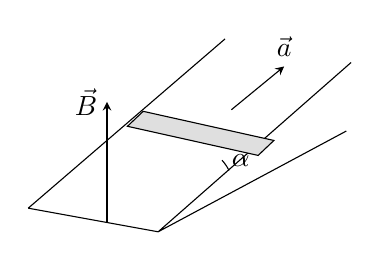
\begin{tikzpicture}[>=stealth]

\draw (0,.3)--(1.65,0)--(4.1,2.15) (0,.3)--(2.5,2.45) (1.65,0)--(4.04,1.28);
\draw (2.55,.78) arc(27:42:.6) node[right]{$\alpha$};
\draw[fill=gray!25] (1.26,1.34)--(2.92,.97)--(3.12,1.16)--(1.46,1.53)--cycle;
\draw[->] (2.58,1.55)--(3.25,2.1) node[above]{$\vec a$};\draw[->] (1,.13)--(1,1.65) node[left]{$\vec B$};
\end{tikzpicture}\end{center}

По стержню протекает ток I. Угол наклона плоскости $\alpha = 30 ^\circ.$ Отношение массы стержня к его длине $\frac{m}{L} =0{,}1\,\text{кг/м}.$ Модуль индукции магнитного поля $B = 0{,}2\,\text{Тл}.$ Ускорение стержня $a = 1{,}9\,\text{м/с} ^2 .$ Чему равна сила тока в стержне?
}{
\smallskip\noindent\textbf{Решение}\par
\begin{center}\begin{tikzpicture}[>=stealth]

\draw (0,0)--(3.2,0);\draw[->] (0,0)--(3.2,1.85) node[right]{$x$};\draw (.65,0)arc(0:30:.65)node[midway,right]{$\alpha$};
\draw[fill=gray!20,rotate=30] (1.1,0)rectangle(2,.43);
\coordinate (M) at (1.34,.79);\draw[->] (M)--(2.68,.79)node[right]{$\vec F_{\!\text{А}}$};
\draw[->] (M)--(.71,1.88) node[above]{$\vec N$};\draw[->] (M)--(1.34,-.55) node[below]{$m\vec g$};
\end{tikzpicture}\end{center}
$1$.  На рисунке показаны силы, действующие на стержень с током:
—  сила тяжести $m\vec{g},$ направленная вертикально вниз; 
—  сила реакции опоры $\vec{N},$ направленная перпендикулярно к наклонной плоскости;
—  сила Ампера $\vec F_{\,\text{А}},$ направленная горизонтально вправо, что вытекает из условия задачи.
$2$.  Модуль силы Ампера $F_{\,\text{А}}=IBL \sin \beta ,$ где  угол между направлением тока и вектором магнитной индукции $\sin \beta =1.$
$3$.  Систему отсчета, связанную с наклонной плоскостью, считаем инерциальной. Для решения задачи достаточно записать второй закон Ньютона $\vec{N} + \vec F_A + m \vec{g}=m \vec{a} .$ 
В проекциях на ось х (см. рис.):

\[ma= - mg \sin \alpha + IBL \cos \alpha .\]

Отсюда находим $I= \frac{m ( a + g \sin \alpha )}{LB \cos \alpha} = \frac{0{,}1 \cdot ( 1{,}9 + 10 \cdot \sin 30 ^\circ )}{0{,}2 \cdot \cos 30 ^\circ} \approx 4\,\text{А}.$

Ответ: $I\approx 4\,\text{А}.$
}

% Source sdamgia-20041: https://phys-ege.sdamgia.ru/problem?id=20041
\BankTask{sdamgia-20041}{
\begin{center}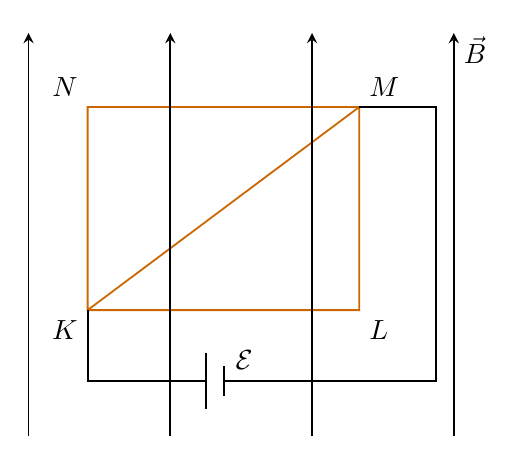
\begin{tikzpicture}[>=stealth,line width=.65pt]\draw[orange!80!black](.75,.9)rectangle(4.2,3.48) (.75,.9)--(4.2,3.48);\draw(.75,.9)--(.75,0)--(2.25,0) (2.48,0)--(5.17,0)--(5.17,3.48)--(4.2,3.48);\draw(2.25,-.35)--(2.25,.35) (2.48,-.19)--(2.48,.19);\node[above right]at(2.5,.02){$\mathcal E$};\foreach \x in {0,1.8,3.6,5.4}{\draw[->](\x,-.7)--(\x,4.42);} \node[below left]at(.75,.9){$K$};\node[above left]at(.75,3.48){$N$};\node[above right]at(4.2,3.48){$M$};\node[below right]at(4.2,.9){$L$};\node[right]at(5.4,4.2){$\vec B$};\end{tikzpicture}\end{center}

Из медной проволоки с удельным сопротивлением $\rho$  =  $1{,}7$ · $10^{-8}$ Ом · м и площадью поперечного сечения S  =  $0{,}2\,\text{мм}^{2}$ изготовлен прямоугольный контур KLMN с диагональю KM (см. рис.). Стороны прямоугольника KL  =  $l_{1}$  =  $20\,\text{см}$ и LM  =  $l_{2}$  =  $15\,\text{см}$. Контур подключили за диагональ к источнику постоянного напряжения с ЭДС $\mathcal{E}$  =  $1{,}4\,\text{В}$ и поместили в однородное магнитное поле с индукцией В  =  $0{,}1$ Тл, параллельной сторонам KN и LM. С какой результирующей силой магнитное поле действует на контур? Сделайте рисунок с указанием сил, действующих на контур. Внутренним сопротивлением источника пренебречь.
}{
\smallskip\noindent\textbf{Решение}\par
\begin{center}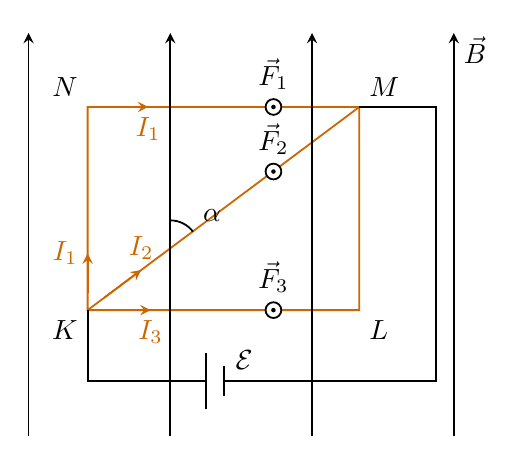
\begin{tikzpicture}[>=stealth,line width=.65pt]\draw[orange!80!black](.75,.9)rectangle(4.2,3.48) (.75,.9)--(4.2,3.48);\draw(.75,.9)--(.75,0)--(2.25,0) (2.48,0)--(5.17,0)--(5.17,3.48)--(4.2,3.48);\draw(2.25,-.35)--(2.25,.35) (2.48,-.19)--(2.48,.19);\node[above right]at(2.5,.02){$\mathcal E$};\foreach \x in {0,1.8,3.6,5.4}{\draw[->](\x,-.7)--(\x,4.42);}\draw[->,orange!80!black](.75,1.12)--(.75,1.62)node[left]{$I_1$};\draw[->,orange!80!black](1,3.48)--(1.52,3.48)node[below]{$I_1$};\draw[->,orange!80!black](.96,1.057)--(1.43,1.409)node[above]{$I_2$};\draw[->,orange!80!black](.99,.9)--(1.55,.9)node[below]{$I_3$};\foreach \x/\y/\i in {3.11/3.48/1,3.11/2.66/2,3.11/.9/3}{\draw[fill=white](\x,\y)circle(.1);\fill(\x,\y)circle(.029);\node[above]at(\x,\y+.09){$\vec F_{\i}$};}\draw(1.8,2.04)arc(90:37:.36)node[above right]{$\alpha$};\node[below left]at(.75,.9){$K$};\node[above left]at(.75,3.48){$N$};\node[above right]at(4.2,3.48){$M$};\node[below right]at(4.2,.9){$L$};\node[right]at(5.4,4.2){$\vec B$};\end{tikzpicture}\end{center}

$1$.  При подключении контура к источнику напряжения по его сторонам и диагонали потекут токи $I_{1}$, $I_{2}$ и $I_{3}$ (см. рис.). Проводники KNM, KLM и KM соединены параллельно, следовательно, $I_1=I_3= \frac{\mathcal{E}}{R_1}$ и $I_2= \frac{\mathcal{E}}{R_2} ,$ где $R_1=\rho \cdot \frac{l_1 + l_2}{S}$ и $R_2=\rho \cdot \frac{l}{S}$ $( KM=l= \sqrt{l_1 ^2 + l_2 ^2} )$  — сопротивления соответствующих проводников.
$2$.  Со стороны магнитного поля на проводники KL и NM, перпендикулярные индукции магнитного поля, а также на диагональ KM действуют силы Ампера: $F_1=F_3=BI_1l_1,$ и $F_2=BI_2l \sin \alpha ,$ где $\sin \alpha = \frac{l_1}{l} .$ По правилу левой руки силы Ампера параллельны друг другу и направлены к наблюдателю, на проводники KN и ML сила Ампера не действует. Таким образом, результирующая сила $F = 2F_1 + F_2.$
$3$.  Выполняя преобразования, получим:

$F_1= \frac{B\mathcal{E} Sl_1}{\rho ( l_1 + l_2 )}$ и $F_2= \frac{B\mathcal{E} Sl_1}{\rho \sqrt{l_1 ^2 + l_2 ^2}} .$

В итоге:

$F=2F_1 + F_2=2 \frac{B\mathcal{E} Sl_1}{\rho ( l_1 + l_2 )} + \frac{B\mathcal{E} Sl_1}{\rho \sqrt{l_1 ^2 + l_2 ^2}} = \frac{B\mathcal{E} Sl_1}{\rho} ( \frac{2}{l_1 + l_2} + \frac{1}{\sqrt{l_1 ^2 + l_2 ^2}} ) =$

$= \frac{0{,}1 \cdot 1{,}4 \cdot 0{,}2 \cdot 10 ^{ - 6 } \cdot 0{,}2}{1{,}7 \cdot 10 ^{ - 8 }} ( \frac{2}{0{,}2 + 0{,}15} + \frac{1}{\sqrt{0{,}2 ^2 + 0{,}15 ^2}} ) =3{,}2 \,\text{Н}.$

Ответ: F  =  $3{,}2$ Н.
}


% Source B65453: https://ege.fipi.ru/bank/questions.php?search=1&proj=BA1F39653304A5B041B656915DC36B38&qid=B65453
\BankTask{B65453}{
По прямолинейному проводнику длиной \(50\,\text{см}\), расположенному в однородном магнитном поле с индукцией \(0{,}5\,\text{Тл}\) перпендикулярно линиям индукции поля, течёт ток \(4\,\text{А}\). Определите силу Ампера, действующую на проводник. (в $\text{Н}$).
}{
\smallskip\noindent\textbf{Решение от GPT}\par
Сила Ампера равна \(F=BIl\sin\alpha\). При \(l=0{,}50\,\text{м}\) и \(\alpha=90^\circ\):
\[
F=0{,}5\cdot4\cdot0{,}50=1\,\text{Н}.
\]
Ответ: \(1\,\text{Н}\).
}

% Source 5ED18A: https://ege.fipi.ru/bank/questions.php?search=1&proj=BA1F39653304A5B041B656915DC36B38&qid=5ED18A
\BankTask{5ED18A}{
Прямолинейный проводник длиной \(0{,}2\,\text{м}\), по которому течёт электрический ток, расположен в однородном магнитном поле с индукцией \(B=0{,}6\,\text{Тл}\) под углом \(30^\circ\) к вектору \(\vec{B}\). Сила, действующая на проводник со стороны магнитного поля, равна \(0{,}12\,\text{Н}\). Какова сила тока в проводнике (в $\text{А}$)?
}{
\smallskip\noindent\textbf{Решение от GPT}\par
Из формулы силы Ампера \(F=BIl\sin\alpha\) получаем
\[
I=\frac{F}{Bl\sin\alpha}=\frac{0{,}12}{0{,}6\cdot0{,}2\cdot\sin30^\circ}=2\,\text{А}.
\]
Ответ: \(2\,\text{А}\).
}

% Source 91A4F6: https://ege.fipi.ru/bank/questions.php?search=1&proj=BA1F39653304A5B041B656915DC36B38&qid=91A4F6
\BankTask{91A4F6}{
Прямолинейный проводник длиной $L$, по которому протекает ток $I$, помещён в однородное магнитное поле перпендикулярно линиям индукции $\vec B$. Во сколько раз уменьшится сила Ампера, действующая на проводник, если его длину увеличить в $3$ раза, индукцию магнитного поля уменьшить в $6$ раз, а силу тока в проводнике поддерживать прежней?
}{
\smallskip\noindent\textbf{Решение от GPT}\par
$F=BIL$, поэтому $F_2/F_1=(B_2/B_1)(L_2/L_1)=\frac16\cdot3=\frac12$. Ответ: в $2$ раза.
}

% Source D0F00F: https://ege.fipi.ru/bank/questions.php?search=1&proj=BA1F39653304A5B041B656915DC36B38&qid=D0F00F
\BankTask{D0F00F}{
Два прямолинейных проводника помещены в однородное магнитное поле перпендикулярно линиям индукции магнитного поля $\vec B$. Длина первого проводника равна $L$, сила протекающего по нему тока равна $I$. Длина второго проводника равна $0{,}8L$, сила протекающего по нему тока равна $0{,}5I$. Чему равно отношение $F_2/F_1$ модулей сил Ампера, действующих на проводники?
}{
\smallskip\noindent\textbf{Решение от GPT}\par
$F=BIL$, поэтому $F_2/F_1=(I_2/I_1)(L_2/L_1)=0{,}5\cdot0{,}8=0{,}4$. Ответ: $0{,}4$.
}

% Source 56DF4A: https://ege.fipi.ru/bank/questions.php?search=1&proj=BA1F39653304A5B041B656915DC36B38&qid=56DF4A
\BankTask{56DF4A}{
Алюминиевый проводник $\text{АБ}$ подвешен на тонких медных проволочках к деревянной балке и подключён к источнику постоянного напряжения так, как показано на рисунке. Справа от проводника находится южный полюс постоянного магнита. Ползунок реостата плавно перемещают влево.
\begin{enumerate}
\item Сопротивление внешней цепи увеличивается.
\item Линии индукции магнитного поля, созданного магнитом вблизи проводника $\text{АБ}$, направлены влево.
\item Сила тока, протекающего через проводник $\text{АБ}$, уменьшается.
\item Сила Ампера, действующая на проводник $\text{АБ}$, увеличивается.
\item Сила натяжения проволочек, на которых подвешен проводник $\text{АБ}$, увеличивается.
\end{enumerate}
\begin{center}
\begin{tikzpicture}[book diagram,x=0.027cm,y=0.027cm,line cap=round,line join=round]
\draw[line width=1pt] (1,141)--(134,207);
\foreach \x in {4,14,...,114}{\draw[thin] (\x,{140+0.5*\x})--({\x-13},{153+0.5*\x});}
\draw (20,151)--(20,20);
\draw (114,187)--(114,70);
\fill (20,140) circle (1.7);
\fill (114,186) circle (1.7);
\draw[line width=2pt] (20,20)--(114,70);
\node[left] at (15,30) {$\text{А}$};
\node[right] at (114,76) {$\text{Б}$};
\draw (20,140)--(142,140)--(171,155);
\draw[line width=0.9pt] (171,133)--(171,176);
\draw[line width=0.9pt] (178,145)--(178,164);
\node at (156,132) {$+$};
\node at (193,149) {$-$};
\draw (178,155)--(236,186)--(187,186);
\draw (114,186)--(161,186);
\draw (161,180) rectangle (187,192);
\draw (198,186)--(198,207)--(171,207);
\draw[-{book tip}] (171,207)--(171,193);
\draw (107,1)--(225,1)--(265,20)--(265,58)--(143,58)--(107,39)--cycle;
\draw (107,39)--(225,39)--(265,58);
\draw (225,1)--(225,39);
\draw (167,1)--(167,39)--(202,58);
\node[font=\Large] at (122,20) {$S$};
\node[font=\Large] at (210,20) {$N$};
\end{tikzpicture}
\end{center}
}{
\smallskip\noindent\textbf{Решение от GPT}\par
При перемещении ползунка влево рабочая длина реостата и сопротивление внешней цепи уменьшаются, поэтому ток возрастает: утверждения 1 и 3 неверны. Вблизи южного полюса магнитное поле направлено к нему, то есть вправо, поэтому утверждение 2 неверно. Ток идёт по проводнику от $\text{А}$ к $\text{Б}$, и по правилу левой руки сила Ампера направлена вниз; её модуль $F_A=BIl$ возрастает, поэтому утверждение 4 верно. Для равновесия суммарная вертикальная сила натяжения равна $mg+F_A$ и также возрастает, поэтому утверждение 5 верно. Ответ: $45$.
}

% Source 33064: https://phys-ege.sdamgia.ru/problem?id=33064
\BankTask{33064}{
Три параллельных длинных прямых проводника $1$, $2$ и $3$ расположены на одинаковом расстоянии а друг от друга (см. рис. а и б). В каждом проводнике протекает электрический ток силой I. Токи во всех проводниках текут в одном направлении. Определите направление результирующей силы, действующей на проводник $1$ со стороны проводников $2$ и $3$. Сделайте рисунок, указав в области проводника $1$ векторы магнитной индукции полей, созданных проводниками $2$ и $3$, вектор магнитной индукции результирующего магнитного поля и вектор результирующей силы. Ответ поясните, опираясь на законы электродинамики.

\begin{center}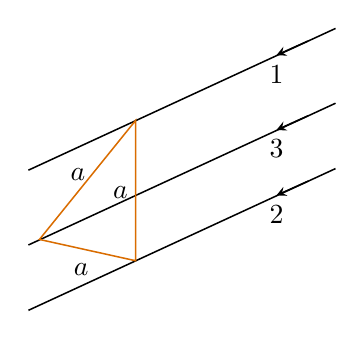
\begin{tikzpicture}[>=stealth,line width=.55pt]\draw(-.5,0)--(3.4,1.8) (-.5,.83)--(3.4,2.63) (-.5,1.78)--(3.4,3.58);\draw[orange!85!black](.86,.63)--(.86,2.41)--(-.36,.9)--cycle;\foreach \y/\i in {0/2,.83/3,1.78/1}{\draw[->](3.05,\y+1.64)--(2.65,\y+1.46)node[below]{$\i$};}\node at(.67,1.49){$a$};\node at(.13,1.73){$a$};\node at(.17,.52){$a$};\end{tikzpicture}\end{center}
Рис. а)

\begin{center}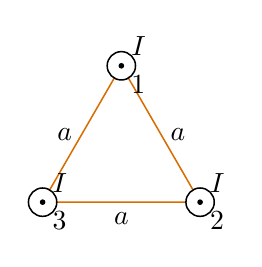
\begin{tikzpicture}[>=stealth,line width=.55pt]\draw[orange!85!black](0,0)--(2,0)--(1,1.732)--cycle;\foreach \x/\y/\i in {0/0/3,2/0/2,1/1.732/1}{\draw[fill=white](\x,\y)circle(.18);\fill(\x,\y)circle(.036);\node[below right]at(\x,\y){$\i$};\node[above right]at(\x,\y){$I$};}\node[below]at(1,0){$a$};\node[left]at(.5,.86){$a$};\node[right]at(1.5,.86){$a$};\end{tikzpicture}\end{center}
Рис. б)
}{
\smallskip\noindent\textbf{Решение}\par
На проводник $1$ со стороны проводников $2$ и $3$ действует результирующая сила, направленная вниз (см. рис.).
\begin{center}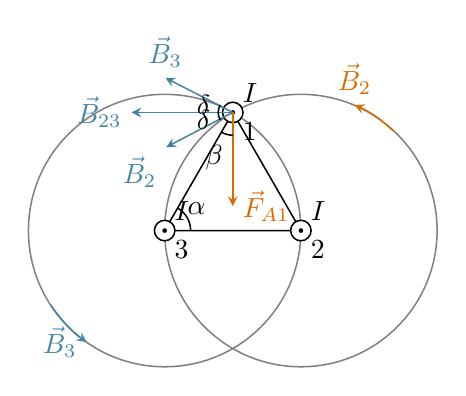
\begin{tikzpicture}[>=stealth,line width=.55pt]\draw[gray](0,0)circle(1.73) (1.73,0)circle(1.73);\draw(0,0)--(.865,1.5)--(1.73,0)--cycle;\foreach \x/\y/\i in {0/0/3,1.73/0/2,.865/1.5/1}{\draw[fill=white](\x,\y)circle(.13);\fill(\x,\y)circle(.03);\node[below right]at(\x,\y){$\i$};\node[above right]at(\x,\y){$I$};}\draw[->,cyan!60!black](.865,1.5)--(.01,1.94)node[above]{$\vec B_3$};\draw[->,cyan!60!black](.865,1.5)--(.02,1.06)node[below left]{$\vec B_2$};\draw[->,cyan!60!black](.865,1.5)--(-.42,1.5)node[left]{$\vec B_{23}$};\draw[->,orange!85!black](.865,1.5)--(.865,.31)node[right]{$\vec F_{A1}$};\draw[->,orange!85!black](2.91,1.26)arc(46:66:1.73)node[above]{$\vec B_2$};\draw[->,cyan!60!black](-1.45,-.94)arc(213:235:1.73)node[left]{$\vec B_3$};\draw(.68,1.5)arc(180:211:.185)node[left]{$\delta$};\draw(.68,1.5)arc(180:149:.185)node[left]{$\delta$};\draw(.33,0)arc(0:60:.33)node[right]{$\alpha$};\draw(.72,1.25)arc(240:270:.29)node[below left]{$\beta$};\end{tikzpicture}\end{center}
Вокруг проводников $2$ и $3$ возникает магнитное поле, линии индукции которого являются окружностями. Направление линий индукции магнитного поля определяется правилом буравчика. Вектор магнитной индукции результирующего поля в области проводника $1$ определяется принципом суперпозиции полей $\vec{B}_23=\vec{B}_2 + \vec{B}_3, \,\text{где}$ $\vec{B}_2$ и $\vec{B}_3$ − векторы индукции магнитных полей, созданных проводниками $2$ и Поскольку проводник $1$ находится на одинаковом расстоянии a от каждого из проводников $2$ и $3$, по проводникам протекают токи одинаковой силы, то $|\vec{B}_2|=|\vec{B}_3|=B.$
Из геометрических построений видно, что угол между векторами $\vec{B}_2$ и $\vec{B}_3$ составляет $60$°, значит, $\,\text{дельта} =30 ^\circ .$ Следовательно, вектор магнитной индукции $\vec{B}_23$ направлен горизонтально влево. Со стороны результирующего поля на проводник $1\,\text{с}$ током действует сила Ампера F$_{A1}$, направление которой определяется правилом левой руки. Таким образом, результирующая сила, действующая на проводник $1$ со стороны проводников $2$ и $3$, направлена вертикально вниз.

Ответ: на проводник $1$ со стороны проводников $2$ и $3$ действует результирующая сила, направленная вниз.
}

% Source 35184: https://phys-ege.sdamgia.ru/problem?id=35184
\BankTask{35184}{
\begin{center}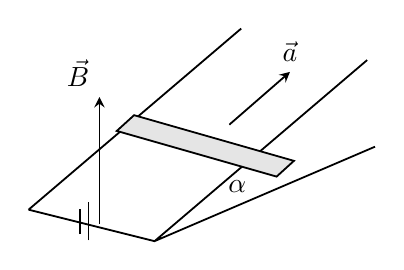
\begin{tikzpicture}[>=stealth,line width=.65pt]\draw (0,0)--(1.6,-.4)--(4.3,1.9) (0,0)--(2.7,2.3) (1.6,-.4)--(4.4,.8);\draw[fill=gray!20] (1.12,1)--(3.15,.42)--(3.37,.62)--(1.34,1.2)--cycle;\draw[->] (.9,-.18)--(.9,1.43) node[above left]{$\vec B$};\draw[->] (2.55,1.08)--(3.32,1.75) node[above]{$\vec a$};\draw (.65,-.31)--(.65,.01) (.76,-.39)--(.76,.1);\node at (2.65,.3){$\alpha$};\end{tikzpicture}\end{center}

 Горизонтальный проводящий стержень прямоугольного сечения поступательно движется с ускорением вверх по гладкой наклонной плоскости в вертикальном однородном магнитном поле (см. рис.). По стержню протекает ток $I=4\,\text{А}.$ Угол наклона плоскости $\alpha =30 ^\circ.$ Отношение массы стержня к его длине $\frac{m}{L} =0{,}1\,\text{кг/м}.$ Модуль индукции магнитного поля $B=0{,}2\,\text{Тл}.$ Чему равно ускорение стержня?
}{
\smallskip\noindent\textbf{Решение}\par
\begin{center}\begin{tikzpicture}[>=stealth,line width=.65pt]\draw (0,0)--(4,0) (0,0)--(3.4,1.95);\draw (.48,0) arc (0:30:.48) node[right]{$\alpha$};\draw[fill=gray!20,rotate=30] (1.45,0) rectangle (2.45,.55);\coordinate (o) at (1.55,1.2);\draw[->](o)--++(2.25,1.3)node[above]{$x$};\draw[->](o)--++(-1.1,1.9)node[left]{$y$};\draw[->,thick](o)--++(-.5,.87)node[below left]{$\vec N$};\draw[->,thick](o)--++(1.5,0)node[right]{$\vec F_{\text{А}}$};\draw[->,thick](o)--++(0,-1)node[below]{$m\vec g$};\draw (2.12,1.2) arc (0:30:.57);\node at (2.28,1.38){$\alpha$};\draw (1.55,.58) arc (-90:-60:.62);\node at (1.89,.5){$\alpha$};\end{tikzpicture}\end{center}

На стержень действуют сила тяжести mg, сила Ампера $F_{A}$ и сила реакции опоры N. Изобразим эти силы на рисунке.
По второму закону Ньютона $m\vec{g} + \vec{N} + \vec F_A=m\vec{a}.$
В проекции на выбранную ось Oх:

\[F_A \cos \alpha - mg \sin \alpha =ma.\]

Сила Ампера находится по формуле $F_A = BIl \sin \beta ,$ где $\beta$  =  $90$\ensuremath{{}^{\circ}}  — угол между направлением тока и вектором магнитной индукции.
Тогда получаем:

\[ma + mg \sin \alpha = BIl \cos \alpha .\]

Отсюда ускорение стержня равно:

\[a= \frac{BIl \cos \alpha}{m} - g \sin \alpha = \frac{0{,}2 \cdot 4 \cdot \cos 30 ^\circ}{0{,}1} - 10 \cdot 0{,}5\approx 1{,}9 \,\text{м/с} ^2 .\]

Ответ: $1{,}9\,\text{м/с}^{2}$.
}

\end{document}
